\chapter{Related Work}
\label{sec:state_of_the_art}
\INITIAL{T}{he field of data visualization} has existed in some form for as long as data analysis has taken place. The primary purpose of data visualization is of course the effective communication of information through the use of graphics. Across varying fields and time periods, different approaches have been applied to varying degrees of success. Most are familiar with basic forms of information graphics, such as tables or basic charts, but as more data is generated and the economy becomes increasingly information-driven we have seen data visualization expand as a field of study in and of itself. 
 
%%%%%%%%%%%%%%%%%%%%%%%%%%%%%%%%%%%%%%%%%%%%%%%%%%%%%%%%%%%%%%%%%%%%%%%%%%%%
%%%%%%%%%%%%%%%%%%%%%%%%%%%%%%%%%%%%%%%%%%%%%%%%%%%%%%%%%%%%%%%%%%%%%%%%%%%%
\section{Visualization of Data}
\label{sec:dataviz}
\INITIAL{D}{ata often contains hidden patterns} which are very easily understood by humans, but can be difficult to extract using basic statistical or computational methods. A demonstration of this was famously constructed by Francis Anscombe in his 1973 paper "Graphs in Statistical Analysis" \cite{Anscombe1973}. Known as Anscombe's quartet, this example consists of four data sets containing (x, y) coordinates. Each of these data sets has identical simple statistical summaries (linear regression coefficients, x and y means, x and y variance, and Pearson Correlation Coefficient). When visualized using a simple scatterplot however, each dataset clearly exhibits a unique pattern. Figure \ref{fig:anscombe} shows Anscombe's quartet visualized together. 

%%%%%%%%%%%%%%%%%%
\begin{figure}
	\centering
	\label{fig:anscombe}
	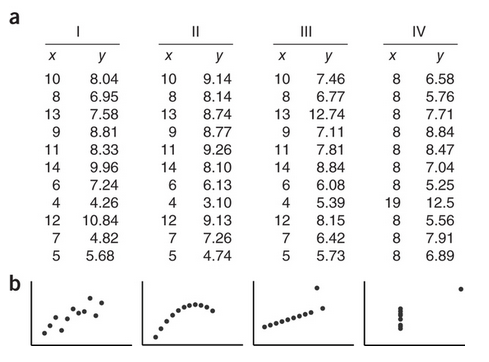
\includegraphics[scale=0.8]{anscombes_quartet.png}
	\caption{Anscombe's Quartet \cite{Shoresh2012}}
\end{figure}
%%%%%%%%%%%%%%%%%%

\paragraph{Tufte}
General purpose visualization techniques have evolved over the past several decades, but often simple techniques still provide the most effective solution. One of the most seminal works in information display is Edward Tufte's "The Visual Display of Quantitative Information"\cite{Tufle1983}. This work provides a summary of several different types of visualizations applied in many fields, but more importantly it sets guidelines as to what makes an effective visualization.

\paragraph{Chart Junk}
Many of the key concepts of Tufte's work revolve around the idea of limiting what he called \emph{chart junk}. Chart junk refers to "useless, non-informative, or information-obscuring elements of information displays"\cite{Tufle1983}. While Tufte acknowledges that using non-data graphics can help to editorialize or provide context for the information being displayed,  it is more important to ensure that data is not distorted in order to fit an aesthetic. 

\paragraph{Data-rich Visualizations}
In addition to limiting non-data information in visualizations, Tufte makes a strong case for the value of data-rich visualizations. Data-rich visualizations are those which include all available information, providing a comprehensive view from which macro trends may emerge. In essence, perhaps at the expense of being able to read individual data points, viewing a complete data set visually may provide insight without need for mathematical analysis. One of many examples of this given in the work is the famous map of central London used by Dr. John Snow to determine the root cause of a cholera outbreak, shown in Figure \ref{fig:snowmap}. By marking the location of cholera deaths with dots and water pumps with crosses it became immediately clear that deaths were clustered around a central pump on Broad Street. Dismantling this pump quickly stopped the deaths. This provides a clear case where a simple graphical analysis proved far more efficient than mathematical computation would have been in determining a causal link.

%%%%%%%%%%%%%%%%%%
\begin{figure}
	\centering
	\label{fig:snowmap}
	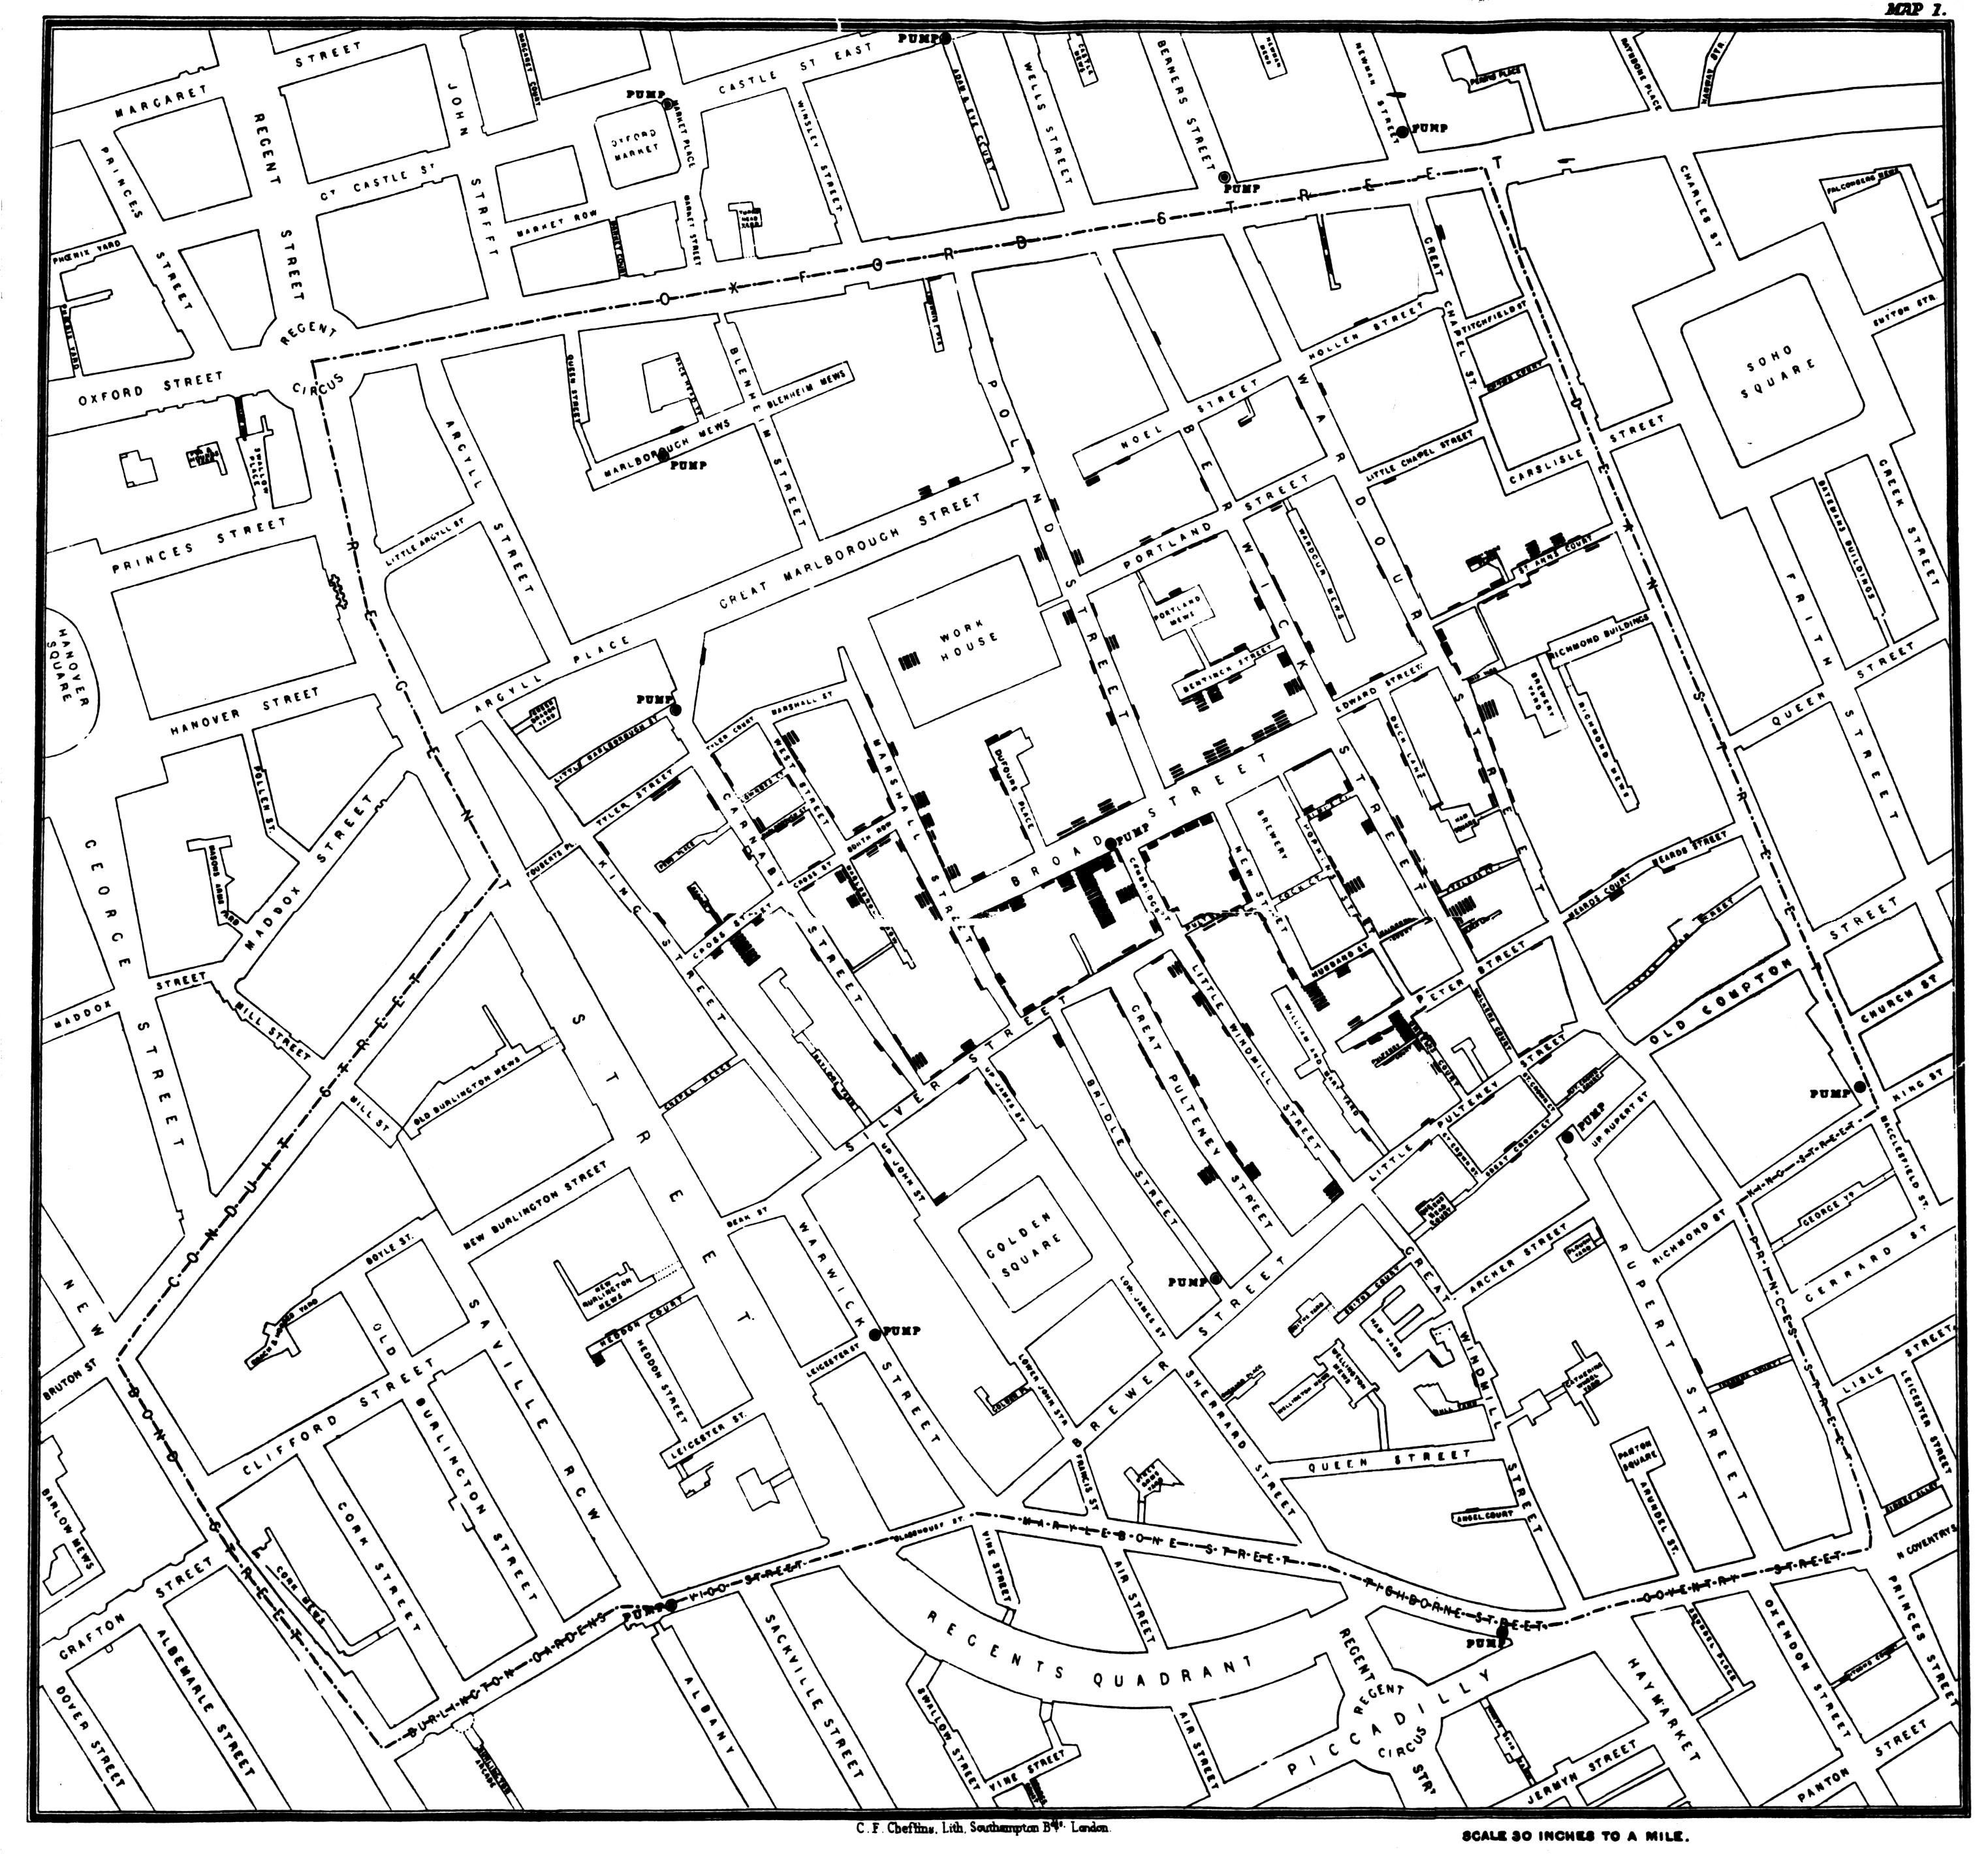
\includegraphics[scale=0.14]{jonsnowmap.jpg}
	\caption{The map used by John Snow to determine the source of a cholera outbreak \cite{Tufle1983}}
\end{figure}
%%%%%%%%%%%%%%%%%%

\paragraph{Dashboards}
A more contemporary area of work which is directly connected to digital display is the concept of a \emph{dashboard}. As defined by Stephen Few, a pre-eminent expert in this area, a dashboard is a single-screen visual display of the information required to achieve a specific set of goals. In a business context, this generally refers to key performance Indicators (KPIs). Such a dashboard is typically generated dynamically, allowing for real-time display of data trends as they occur. An example of such a dashboard as built for the CIO of a generic company is shown in Figure \ref{fig:dashboard}. 

%%%%%%%%%%%%%%%%%%
\begin{figure}
	\centering
	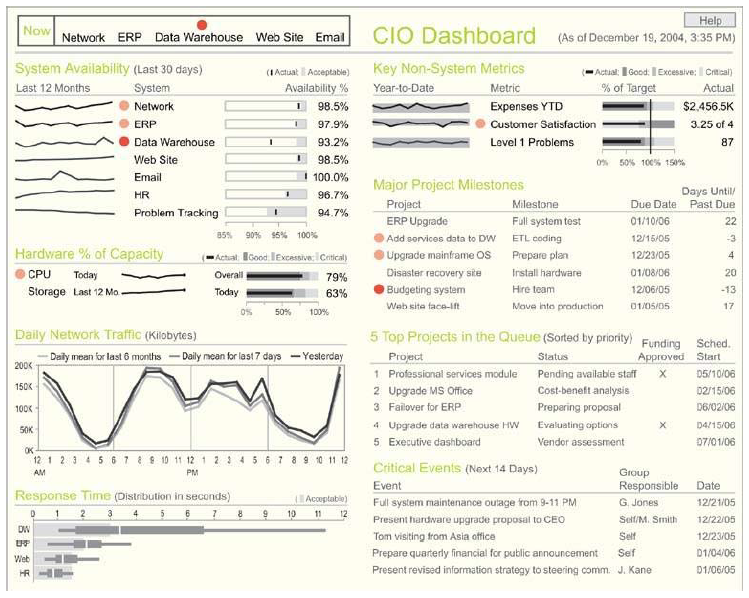
\includegraphics[scale=0.74]{dashboard.png}
	\caption{An example CIO dashboard \cite{Few2006}}
	\label{fig:dashboard}
\end{figure}
%%%%%%%%%%%%%%%%%%

\paragraph{Dashboard constraints}
In Stephen Few's "Information Dashboard Design" \cite{Few2006} a comprehensive guide to the development of dashboards is given. In particular, specific charts and graphics are matched to appropriate use cases and perhaps more importantly, areas in which some visualizations are inappropriate are defined. Beyond being a discussion simply on visual design, interactivity is discussed. The author notes that although the capability to explore data and perform analysis is available, for monitoring purposes it is more appropriate to not allow such features. Though these analyses are often important, it is more crucial to the purpose of a dashboard to display the data in the form that the dashboard was originally designed for. To do otherwise would risk undermining the purpose, which is a focus on optimal display of key metrics.

\paragraph{Evaluation of Visualizations}
Though information visualization has been a very popular research topic for over two decades, there is little in terms of a firm framework by which the success of visualizations can be measured. A review of literature in the area \cite{Amende2010} indicates clearly that the literature is mixed on which evaluation approaches produce actionable results, and to what extent these results are accurate. The variables affecting such an analysis include both an examination of the domain in which data is being visualized, and the intended users of said visualizations. Scientific visualizations will not only demand different features than business visualizations, they will often be examined by users with very different levels of expertise. Exigent variables such as user understanding force data visualization to be examined by somewhat subjective standards in almost all cases. It is difficult to determine if there is a number of hours of productivity saved through the use of a dashboard, for example, if the application of the information therein (and therefore its results) is still heavily dependent on unpredictable external factors such as user expertise. 


\section{In-Situ Processing}
\label{sec:insitu}

\INITIAL{P}{rocessing large quantities of data} has become a common task within many organizations. Data sources such as sensor networks or click streams necessitate handling both massive quantities of information and rapid rates of change. The size of this data presents issues in the efficiency of storage solutions and there are many options for handling such problems \cite{Klasky2011}. Beyond storage, when analysis occurs on large data stores it is often necessary to apply in-situ processing rather than a more thoroughly controlled approach. In-situ analysis allows for results to be obtained quickly by avoiding alterations to the initial state of the data and not isolating it from other active systems. This removes a significant amount of preprocessing that may be involved in an analysis performed on a more controlled data source. Removing preprocessing steps of course increases speed while introducing a number of potential unknown factors which must now be handled in a sort of ad-hoc fashion during the analysis. Because in-situ analysis often occurs on data which is unstructured and not stored in a relational format, it fits hand in hand with analysis platforms which operate on large and unstructured data sets.

\paragraph{Parallel Data Flow Graphs}
There are many platforms which are purpose built for performing analysis on large data sets, the most common of which are based on the MapReduce model of computation. The most widely used analysis platform based on the MapReduce paradigm is Apache Hadoop \cite{ApacheSoftwareFoundation2015}. Hadoop consists of two primary parts: a MapReduce based distributing processing engine, and the Hadoop Distributed File System (HDFS). Conceptually, executing an analysis task in the MapReduce paradigm simply means that the distributed computation task being performed consists of map and reduce operations which are paired to form each step of an overall computation. As more layers of map and reduce steps are added, we are left with a directed acyclic graph of operations which are chained together in a linear way, as can be seen in  Figure \ref{fig:dfg}. This figure represents two MapReduce steps, each of which is separated by a write of the data being operated on to the file system. Systems which utilize the data flow graph model optimize these graphs by grouping together and pipelining operations in order to reduce the overhead and cost as much as possible. Many widely used analysis systems have been built to run on top of or alongside Hadoop.

%%%%%%%%%%%%%%%%%%
\begin{figure}
	\centering
	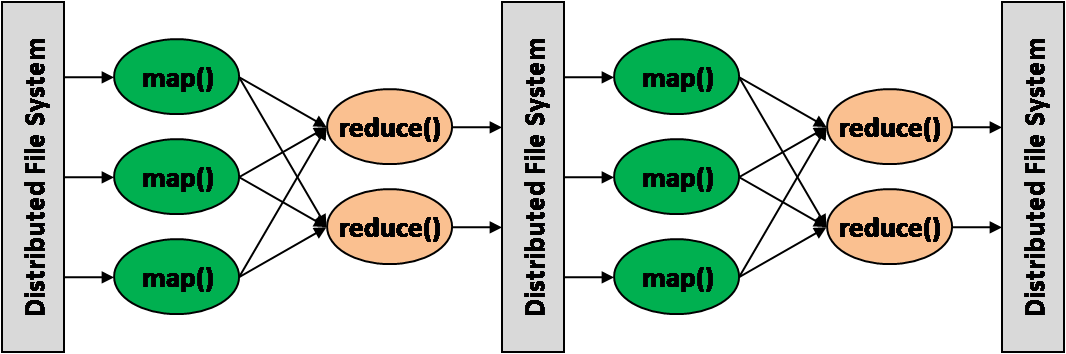
\includegraphics[scale=0.75]{Generic_DFG.png}
	\caption{A generic data flow graph \cite{Ho2008}}
	\label{fig:dfg}
\end{figure}
%%%%%%%%%%%%%%%%%%

\paragraph{Pig}
One of the more popular of these data flow graph based systems is Apache Pig \cite{Gates2009}. Pig consists of two major components: a language, Pig Latin \citep{Olston2008a} in which Pig programs can be written, and the execution environment in which they can be run. Pig acts as a high level tool through which users can develop MapReduce applications for execution in a Hadoop environment. Pig Latin provides users with a simple syntax through which sequential operations can be defined, at which point the execution environment compiles these tasks into Map-Reduce programs for which parallel implementations have already been developed in detail within Hadoop. These sequential tasks are organized into a data flow graph which the system can optimize automatically, greatly simplifying the work of the developer. Additionally, Pig Latin has been designed with extensibility in mind. Developers can write user defined functions in Java, Python, JavaScript, Ruby, or Groovy and then call these functions directly from within a Pig Latin program. Pig was initially developed internally at Yahoo, and quickly became widely applied externally after moving to the Apache foundation a year after its initial development. 

\paragraph{Flink}
Another platform for large scale data processing is Apache Flink. While Pig Latin provides the interface through which developers can work with Pig, Flink is accessed through either a Java or Scala API. For users who are already fluent in either of these languages, this is very convenient. It allows the same extensibility as seen with Pig, where users can write custom functions for execution within an analysis program, but additionally enables the use of native Java and Scala data types. Using these data types without conversion into the key-value pair data format typical of MapReduce removes one more complication for developers and simplifies analysis programs. 

\paragraph{System Differences}
Each of these systems have specific traits related to the way their data flow graphs are generated and optimized. Generally speaking however, the graphs themselves are still functionally similar enough that we can attempt to be generic in the way that this work is applied. 

\section{Visualization of Data Flow Graphs}
\label{sec:dfgviz}

\INITIAL{D}{ata flow graph visualizations} have existed in some form for as long as data flow graphs have been used in analysis systems. However, their use is almost exclusively applied to examining meta-information such as optimization plans. Relatively little work has been done in generating visualizations which help in the understanding of data, as a supplement to the analyses themselves.

\paragraph{IBM System S}
IBM research has developed a stream processing system known as \emph{System S}, which builds processing graphs using predefined operators \citep{Gedik2008} and has included basic visualization of these graphs \cite{Pauw2010}. The visualizations show the DAG of analysis operators and indicate whether the operations have completed through colour coding. Additionally, each operator has a small widget which identifies the tuples which have been passed to or from the operator, as seen in Figure \ref{fig:systemsop}. These tuples can be highlighted in order to show specific data values, and to highlight data dependencies which exist downstream.

%%%%%%%%%%%%%%%%%%
\begin{figure}
	\centering
	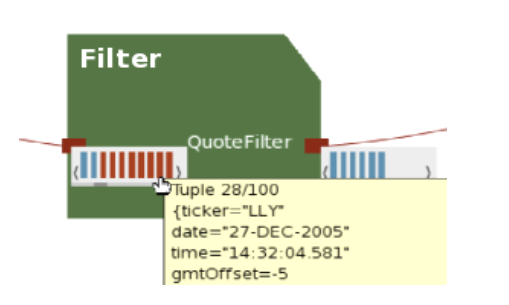
\includegraphics[scale=0.5]{SystemSOperator.png}
	\caption{An executing operator as visualized in IBM's System S 
	\citep{Pauw2010}}
	\label{fig:systemsop}	
\end{figure}
%%%%%%%%%%%%%%%%%%

\paragraph{Retrospective Debugging}
This type of visualization exists primarily to support debugging after some failure has been detected post-analysis. It can be seen in Figure \ref{fig:systemsop} that there are only ten tuples visible at a single time. Though this number can be expanded, this limitation is here because the envisioned use-case consists of a user scrolling through tuples to identify a single suspected problem tuple. While this is very useful for repairing a problem which is found post-analysis, in cases where this computation is very expensive or the problem is particularly unclear after a failure it may not be efficient. 

\paragraph{Lipstick}
Lipstick \citep{Amsterdamer2011}, a workflow provenance model framework built for use with Pig takes a similar approach to that of IBM. Lipstick examines the internals of modules within a data flow in order to determine dependencies between parts of a flow. This approach is used for very much the same debugging cases which are expected within System S, with the addition of an added feature allowing developers to query a dependency graph. These queries allow developers to change parameters of the tuples in the graph in order to undertake "what-if" style analyses. Beyond the analysis options introduced through the querying capabilities of Lipstick however, the added visualization features are relatively simple. Like in System S, single operations change colour to indicate status and the tuples being passed to and from operations are identified. In this case the key difference is that the widget for selecting single tuples from System S is replaced with a simple integer iindicating the quantity of tuples moving through a flow. The exploratory capabilities here are left for queries made against the graphs generated in Lipstick.

\paragraph{Flink Plan Visualizer}
The approach taken by Flink in visualizing the execution of a job is focused less on the provenance on data and operations and more on the organization of the execution plan as decided by the internal optimizer. Depending on the input sizes and other variable factors in a job, the same program may be executed very differently so that optimal performance can be achieved. Because the development API and the way that programs are executed are independent of one another, it is important that a developer have a mechanism through which they can see the execution order as determined by the optimizer. This is provided through the Flink execution plan visualizer \citep{ApacheSoftwareFoundation2014}, which developers can access through their browsers. A form is provided in which users can submit the execution plan in a JSON format (easily extracted from a running job through the development API), at which point it will be neatly rendered on their screen in a format similar to the example shown in FIgure \ref{fig:flinkplan}.

%%%%%%%%%%%%%%%%%%
\begin{figure}
	\centering
	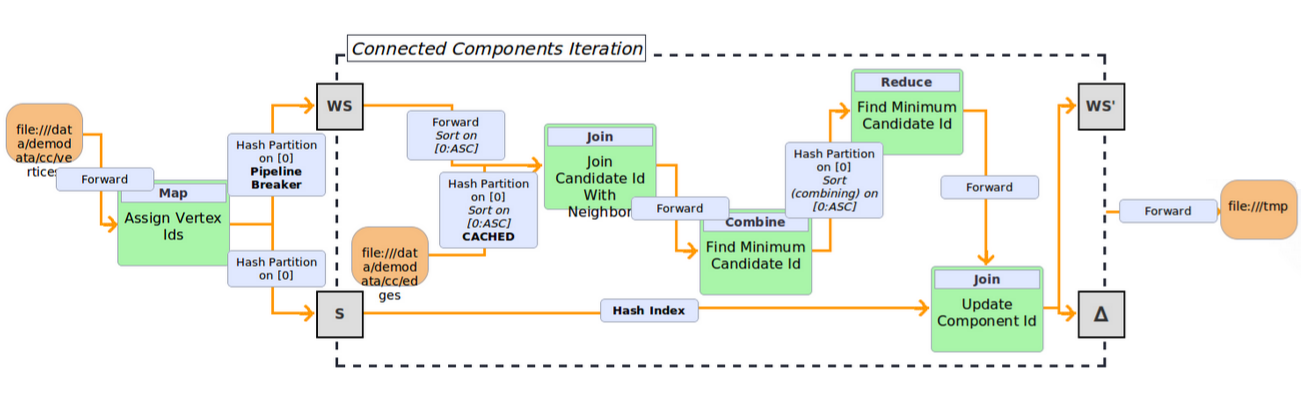
\includegraphics[scale=0.4]{flink_plan.png}
	\caption{An execution plan as seen in the Flink execution plan visualizer	\citep{ApacheSoftwareFoundation2014}}
	\label{fig:flinkplan}	
\end{figure}
%%%%%%%%%%%%%%%%%%


